\documentclass{btswhitepaper}
\title{Smartcoins on the BitShares Blockchain}
\author{
 \IEEEauthorblockN{Fabian~Schuh}
 \IEEEauthorblockA{BitShares Europe, BitShares.eu\\
                   Erlangen, Germany\\
                   Email: \texttt{fabian@bitshares.eu}}
 \and
 \IEEEauthorblockN{Daniel~Larimer}
 \IEEEauthorblockA{Cryptonomex, Cryptonomex.com\\
                   Blacksburg (VA), USA\\
                   Email: \texttt{dan@cryptonomex.com}}%
 \thanks{This work was supported by Cryptonomex and honorable members of the
         bitsharestalk.org community.}
}


\begin{document}
\sloppy
\maketitle

\begin{abstract}%

 This document serves as a detailed and accurate description of so called
 \emph{smartcoins}, often also referred to as \emph{bitassets} or \emph{market
 pegged assets}. These refer to special kinds of tokens that are governed
 autonomously and transparently by the blockchain's internal smartcoin
 framework - a set of smart contracts. This framework enables a variety of
 interesting token types. Prominent examples are \textbf{bitUSD} and
 \textbf{bitCNY} which provide automation and incentives for market
 participants to maintain a high correlation with the value of U.S. Dollar or
 CNY.

\end{abstract}

\section       { Introduction                                     } \label{sec:mpa}
%%%%%%%%%%%%%%%%
% Smartcoins
%%%%%%%%%%%%%%%%
In today's world, crypto-currencies are unique because they are the only type
of digital currency that does not represent a corresponding counterparty
liability. Instead, they are \emph{fungible} and \emph{decentralized} tokens, whose
value is derived from the amount of practical utility (or potential future
utility) perceived by the network of users that support and trade in them.

Not surprisingly, most crypto-currencies suffer from high levels of price
volatility due to many complex factors, such as constantly shifting
public perception and highly speculative and unregulated markets.
Although professional traders tend to appreciate this volatility, so far
it has hindered the widespread adoption of cryptocurrency as a
\emph{practical payment solution}. A crypto-currency that has the
properties and advantages of Bitcoin, but is also capable of maintaining
price parity with a globally adopted currency (e.g. U.S. dollar), would
have incredible high utility for convenient and fast e-commerce.

The BitShares Blockchain offers a solution to this problem by introducing
\emph{smartcoins} - a framework for collateralized, counterparty risk-free loans
that enable token that highly correlate with the valuation of an
underlying asset, such as U.S. Dollar. Said framework is realized by a set of smart contracts
on the blockchain. 

Most prominent example of smartcoins on the BitShares Blockchain are 
\emph{bitUSD} and \emph{bitCNY}, which are smartcoins specific to one particular use
- namely to realize price-stable tokens. It is worth noting that that
price-stable tokens are merely one subset of possiblities within the
smartcoin framework. In literature, smartcoins are also often referred
to as \emph{bitassets} or \emph{market pegged asset}.
\section       { Terminology                                      } In this paper we refer to \emph{smartcoins} as a means for customization of
tokens within a \emph{framework} of smart contracts and parameters as offered
by the BitShares Blockchain. In literature, smartcoins are also often referred
to as \emph{bitassets} or \emph{market pegged asset}.

As such, tokens like \emph{bitUSD}, \emph{bitCNY} and others are merely cases
specific to one particular use.


%\section       { Smartcoin Tokens                                 } Before diving into the mechanics of smartcoins, let us first briefly
review the smartcoin framework and describe which parameters are
available for customization of tokens as well as its autonomous and
transparent nature. Furthermore, we will describe the price feeds which serve
as \emph{oracle} to feed a trusted price into the blockchain.

Last but not least, we would like to address the distinction between publicly
and privately managed smartcoin tokens.

Please note that in most parts of this paper we will often refer to bitUSD or
bitCNY as examples for \emph{price-stable} smartcoins as they are available on
the BitShares Blockchain even though many more use case exist.

%\subsection    { Autonomy and Transparency                        } % Autonomy and Transparency

Every smartcoin comes with a variety of features and autonomously
executed contracting logic. As every blockchain-based smart contract,
this contract autonomously executes according to public data as it
stored on the blockchain.

What does this mean in particular for the smartcoin framework?
If we compare smart contracts with business logic, we realize that 


% Parameters

%\subsection    { Ownership and Responsibilities                   } Alternatively to public smartcoins like the bitUSD, BitShares also offers
entrepreneurs an opportunity to create their own SmartCoins with custom
parameters and a distinct set of price feed producers.

Privatized SmartCoin managers can experiment with different parameters such as
collateral requirements, price feeds, force settlement delays and forced
settlement fees (see \cref{sec:uia:priv}). They also earn the trading fees from
transactions the issued asset is involved in, and therefore have a financial
incentive to market and promote it on the network. The entrepreneur who can
discover and market the best set of parameters can earn a significant profit.
The set of parameters that can be tweaked by entrepreneurs is broad enough that
SmartCoins can be used to implement a fully functional prediction market with a
guaranteed global settlement at a fair price, and no forced settlement before
the resolution date.

Some entrepreneurs may want to experiment with SmartCoins that always trade at
exactly \$1.00 rather than strictly more than \$1.00. They can do this by
manipulating the forced settlement fee continuously such that the average
trading price stays at about \$1.00. By default, BitShares prefers fees set by
the market, and thus opts to let the price float above \$1.00, rather than
fixing the price by directly manipulating the forced settlement fee.


\section       { Mechanics                                        } In the following section, we describe the mechanics of smartcoins in
detail. These include the creation of call orders~\cref{sec:callorder}
for borrowing, settlements in~\cref{sec:settlement} as well as margin
calls~\cref{sec:margincall}.

\subsection    { Feeds                                            } \label{sec:feeds}

The blockchain needs to be aware of a fair valuation of the token and
its collateral (think, the value of BTS in USD) in order to enable
margin calls and allow for settlements to convert tokens into the
collateral token (in most cases BTS) at a fair price.

A feed constitutes multiple attributes including
\begin{description}
 \item[price] of the token with respect to the collateral of the smartcoin,
  e.g., the BTS price in USD.
 \item[maximum short squeeze ratio]: Given that margin calls are force to buy
  in the markets, this ratio defines the upper bound for the premium that needs
  to be paid in case of a margin call.
 \item[maintenance collateral ratio]: This parameter defines the minimum
  required collateral as a ratio between the token and the value of the
  collateral denoted in token. If the collateral ratio of any call order (a
  borrow position) comes below this ratio, a margin call for the call order is
  triggered.
\end{description}

These parameters are in the hands of the group selected by the owner of the
smartcoin. Only those are allowed to produce valid price feeds for a particular
smartcoin. In case of \emph{bitUSD}, \emph{bitCNY} and others, the owner of the
token is the committee, a group of people elected by the BTS holders. Here, the
group of feed producers coincides with the group of block producers (i.e.
\emph{witnesses})

These $N$ trusted witnesses can be constantly reviewed as all feeds are put on
the blockchain. Hence, misbehaving witnesses can be identified, fired from
their revenue generating witness position and lose their reputation.

Additionally, to prevent manipulation of the price feed (and the other
parameters), $N$ witnesses have to be elected that can all produce their feeds
independently. Having a set of $N$ feeds $p_i,\;1<i<N$ for an arbitrary MPA on
the blockchain, the protocol obtains a value $\tilde{p}$ by the use of the
\emph{median} according to:
\begin{align}
 x &= \operatorname{sort}(p[i])\\
 \tilde p &=\begin{cases}
   x[\frac{N+1}{2}]                                               & N \text{ odd}\\
   \frac {1}{2}\left(x[{\frac{N}{2}}] + x[\frac{N}{2} + 1]\right) & N \text{ even.}
 \end{cases}
\end{align}
Hence, the price, as well as the other parameters, are resistant against
misbehaving witnesses in that only a majority of feed publishers can manipulate
the outcome of the median. In practice, any unintentional feed \emph{error} is
thus balanced around the median value.




%% Continue here


Obviously, the shareholders are required to constantly monitor the published
prices of their witnesses and should make a public note about any
discrepancies. This is similar to traditional \emph{quality management} for the
\emph{Smart Coin} products (e.g. bitUSD) and BitShares system can offer a paid
position to perform this service.

There is always concern of price manipulation. Someone with a large amount of
money on both sides of a trade can use their funds to manipulate the markets
and thus the price feed. If the amount of money they lose manipulating the
markets is less than the amount of money they can gain by manipulating the
price feed, then it will be profitable to manipulate the market at the expense
of either the BitUSD longs or the shorts. A low collateralized short that sees
a large force or global settlement order requested can attempt to manipulate
the markets and thus the feed against the BitUSD holder.

The risk of price manipulation should be priced into the premium on BitUSD
charged by the shorts, and thus should already be priced into the market. If
price manipulation became a serious problem that caused very high premiums,
then it could be addressed by the price feed producers, who can adopt a moving
average over wider time windows to increase the difficulty of short-term
manipulation. A variety of algorithms could be used to estimate a \emph{fair
price}\footnote{``fair'' for honest market participants.} that keeps BitUSD
valued at least \$1.00.

In practice, a feed producer can observe the BitUSD:USD market as an indicator
on which way to adjust the feed. Generally speaking, the strategy that the feed
producers adopt for controlling the feed should be public knowledge, because
the shorts will ultimately rely on it. For the feed producers to change
strategies in unpredictable ways could cause losses to both longs and shorts.
Fortunately, it is assumed that shareholders primarily approve complying feed
producers and quickly fire misbehaving feed providers.


% parameters:
%%%%%%%%%%%%%%%
% maximum_short_squeeze_ratio
% maintenance_collateral_ratio
% price
% minumin feeds
% force_settlement_delay_sec
% force_settlement_offset_percent
% maximum_force_settlement_volume
% short_backing_asset

\subsection    { Collateralization                                } \label{sec:collateral}

As previously mentioned, the collateral is used to secure the debt of a
collateralized loan.
 While all regular assets on the BitShares Blockchain can
technically be used as collateral asset for a smart coin, most smartcoins
use the core native token BTS.
Collateral needs to be provided in order to borrow smartcoins from the
blockchain. The provided collateral will be locked away and can only be
redeemed back when clearing the debt with the blockchain. 
Additional, the collateral can be increased freely at any time to improve the
so called collateral ratio. It can also be reduced, however with the limitation
that the collateral ratio is greater than the collateral maintenance ratio.

Even though the collateral is locked and tied to the user's account, other uses
may obtain your collateral in parts of fully by so called \emph{settlements}
(see below).


\subsection    { Call Orders                                      } \label{sec:callorder}

\subsection    { Settlement                                       } \label{sec:settlement}

% Collateral swap
% http://www.marketswiki.com/wiki/Collateral_swap


\subsection    { Margin Calls                                     } \label{sec:margincall}

However, since markets do not have all their liquidity at the spot or feed
price the blockchain needs a back-off and start closing borrow positions
earlier to prevent a loan defaults. For smartcoins, the back-off factor is
called \emph{Maintenance Collateral Ratio (MCR)} and derives the
position-specific \emph{Margin Call Price} (MCP) by:
\begin{align}
 \MCP = \MCR \;\cdot\; \frac{\text{d}}{\text{c}}
\end{align}

The \MCR\ is a asset-specific parameter defined by the feed providers which can
change to adept to market conditions but is guaranteed to be above $1$. It is
derived from the median of the proposed \MCR s of the feed producers such that
only the majority of feed producers can manipulate this parameter. The \MCR\ implies 
a margin call price \MCP\, which is the price at which the positions gets liquidated automatically.

\paragraph{Example} A commonly agreed value for the \MCR\ is \num{1.75} or 175\%. With the numbers from the previous example
the the margin call price is derived as follows:
\begin{align}
 \MCP &= 1.75 \;\cdot\; \frac{\SI{100}{USD}}{\SI{2500}{BTS}} \\
      &= \SI{0.07}{USD \per BTS}
\end{align}
If the price feed goes below \SI{0.07}{USD \per BTS}, your position will be
automatically liquidated. A margin call is created by the smart contract, which means that the contract
itself will take the collateral and sell just enough of it to market
participants in the internal exchange to increase the \MCR\ back to its
required minimum~\cite{bsip31}.

However, it is worth noting that there is a protection of call positions
against short squeezes. A short squeeze implies that call positions are being
squeezed out of their positions by forcing them into margin and having the
contract sell the collateral to the market (usually at a loss for the owner of
the call position).

To protect shorts against short squeezes, margin calls only execute
\emph{up to} the short squeeze protection price (\SQP).

The \SQP\ is derived by
\begin{align}
 \SQP = p \;/\; \MSQR
\end{align}

with $p$ denoting the price in the form of \si{debt \per collateral}. 

\paragraph{Example}
With the numbers from previous example and a \MSQR\ of
\SI{110}{\percent}, margin calls would buy in the markets and pay up to
\begin{align}
 \SQP &= \SI{0.07}{USD \per BTS} \;/\; \SI{110}{\percent} \\
      &= \SI{0.077}{USD \per BTS} \\
      &\stackrel{\frown}{=} \SI{12.98}{BTS \per USD}\,.
\end{align}
During a margin call, the orders with the least collateral ratio will be called (liquidated)
first~\cite{bsip34}.

\subsubsection { Calling for insufficient collateral              } \input { content/fp-smartcoins-margincall1 }
\subsubsection { Margin Call Orders                               } \input { content/fp-smartcoins-margincall2 }
\subsubsection { Order of Filling                                 } \input { content/fp-smartcoins-margincall3 }

\subsection    { Global Settlement                                } \label{sec:blackswan}

All guarantees of SmartCoins are subject to the caveat that a SmartCoin can
never be worth more than the collateral backing the \emph{least-collateralized}
short position. All collateral above this maintenance collateral limit is
effectively meaningless when it comes to enforcing the ``peg''. In normal
market conditions, the value of the collateral is always more than sufficient,
but, from time to time, markets can rapidly revalue the collateral.

If this revaluation happens faster than the short positions can be forced to
cover, then all SmartCoins are liquidated at the exchange rate of the least
collateralized short position. This is called a \emph{global settlement} (also refered to as  black swan) event since
the least collateralized position is unable to liquidate itself on the market. At
this point, all positions are automatically force settled and any additional
collateral maintained by the short positions is returned to them. This is similar to an
insolvent bank converting its deposits to equity.

\subsubsection { Call Position Migration                          } \input { content/fp-smartcoins-swan-order  }
\subsubsection { Reviving from Global Settlement                  } \input { content/fp-smartcoins-revive      }

\subsection    { Risks                                            } The current implementation of market pegged assets in the BitShares system is
designed to minimize risk of loss to market pegged asset holders. Short
positions are opened with collateral worth three times the market value of the
asset. The initial collateral is comprised of the BTS paid by the buyer for the
asset and twice this amount of BTS contributed by the short seller. The
collateral requirements and margin triggers were chosen conservatively to
protect the holders of market pegged assets from volatility of the underlying
collateral. Forcing short positions to cover every 30 days provides additional
assurance of short term liquidity. Control over the price feed is distributed
among over 50 separately elected delegates who compile information from
multiple exchange sources. Despite such precautions, it is important to
carefully explore risks of using the system. Risks can be broadly categorized
as value risk, counterparty risk, or systemic risk.

\subsubsection { Collateral Risk                                  } Market pegged assets maintain their price parity due to being backed by
collateral that has an established real world value. When the value of the
collateral falls, the system is designed to react by driving the internal asset
exchange to match the new real world exchange rate and trigger \emph{force
settlements} (also known as margin calls) if necessary.

% First half of the paragraph contains dublicated information from
% fp-mpa-blackswan.tex
However, there exists a possibility that the underlying collateral (BTS) drops
in value so quickly the market pegged assets become under-collateralized. Often
termed a \emph{black swan event} (c.f., \cref{sec:blackswan}), a sudden crash
of BTS value could prevent the system from adjusting in time. In this event,
the full amount of collateral is no longer sufficient to purchase the market
pegged asset back at the new real exchange rate. In such an event, assets may
settle at the price fees and are converted back into the underlying collateral
(BTS). This may expose customers at the volatility risk of BTS. Under normal
conditions, short term market movements, spreads, and fees charged by exchanges
may also affect the potential cost of conversion into and out of market pegged
assets.

\subsubsection { Counterparty Risk                                } Unlike many attempts to create a digital asset that tracks the dollar, market
pegged asset are not an ``\emph{I owe you}'' issued by any entity. For this
reason, it does not rely on a specific counterparty to honor its value (unless
you choose to view the software protocol itself as an independent
``counterparty'' entity). 

Although manipulation risk occurs in any market, it is minimized by the open
source and auditable nature of the BitShares system and carefully considered
market rules. MPAs stored on a \emph{centralized} exchange become IOUs and are
subject to counter party risk~\cite{mtgox}. This risk is not a property of the
MPA themselves. We recommend that users never deposit their tokens on an
exchange and instead only use gateways that issue their IOUs onto the BitShares
network. This way you can trade your BitUSD against gateway IOUs without
exposing your BitUSD to counter party risk while in the order book (more
details in \cref{sec:gateway}).

\subsubsection { Systemic Risk                                    } Systemic risk is a catch-all for other risks required to utilize the system.
The primary risk is individuals are responsible for protecting the
cryptographic private keys that sign transactions proving ownership of assets.
These keys must be protected from theft or loss. This risk can be greatly
reduced and virtually eliminated by following best practices.

Systemic risk also includes the possibility of an overlooked fatal flaw in the
open source software or the possibility of large scale failure of global
network infrastructure and should reduce over time.


\section       { Use Case: Price Stability                        } Ever since the bitcoin blockchain initiated the age of decentral public
ledgers, economists and engineers are trying to achieve a stable cryptocurrency
or a price pegged crypto token. The following two subsection want to discuss
the meaning of a ``stable'' currency and show how BitShares want's to fill the
gap.

\subsection    { Definition of Price Stability                    } Before we discuss how BitShares achieves price \emph{stability} we first need to
define what properties make a currency \emph{stable}.

In the U.S., for instance, the Federal Reserve (FED) has a mandate of
\emph{stable prices} and it is almost universally accepted that this is a good
mandate. The same holds true for the Euro with its stability being
\emph{controlled} by the European Central Bank (ECB). Mostly every
country/nation or federation applies a similar concept.

However, it is also widely accepted among many crypto-currency fans that, in
the case of the US dollar, the FED has failed at their mandate because of
monetary inflation and increase in the money supply. Since monetary inflation
is a sustained increase in the general level of prices, it is equivalent to a
decline in purchasing power of money. Hence, a dollar buys less and less over
time. As a result, we see the dollar losing 99\% of its \emph{purchasing power}
since the FED was founded in 1913~(see \cref{fig:monetarybase}). 

\begin{figure}[!htp]
 \centering
 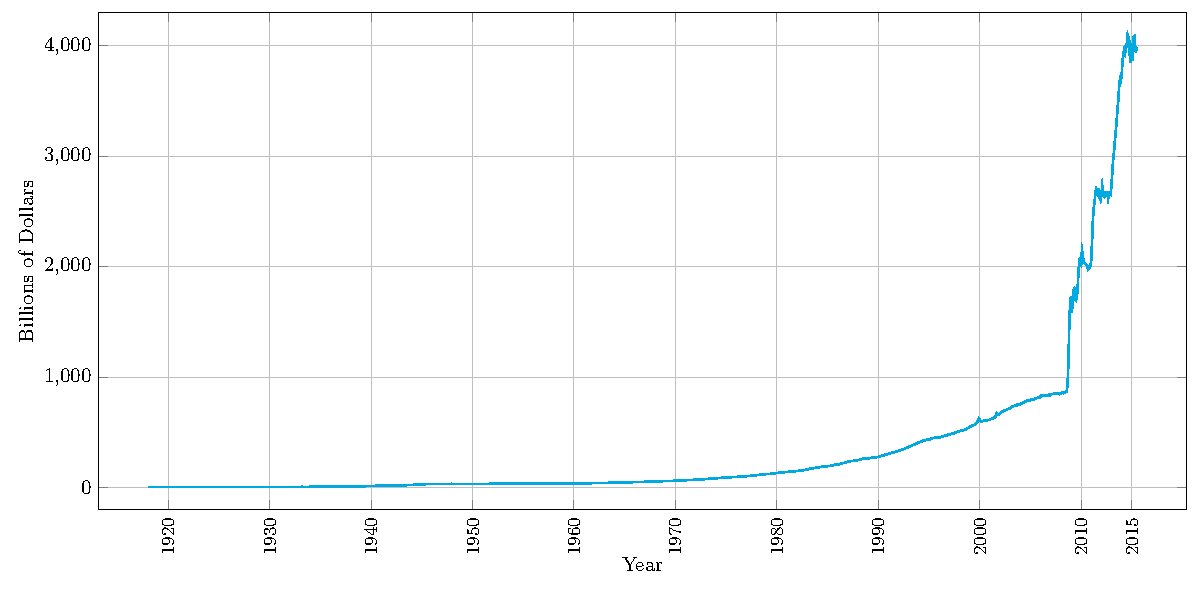
\includegraphics[width=\linewidth]{figures/monetary-base}
 \caption{St. Louis Adjusted Monetary Base~\cite{ambsl}}
 \label{fig:monetarybase}
\end{figure}

The goal of this paper is not to propose a replacement of central banks but to
clarify the terminology in particular with regards to ``stable''
cryptocurrencies. Unfortunately, some people in the cryptocurrency space are
attempting to provide an alternative currency that can achieve the same
mandate. However, since price stability at its heart is the same as \emph{price
fixing}, this is a well known economic fallacy that crypto-currencies should
avoid.

% The goal of the FED price stability mandate is to mask the systematic theft of
% all increases in the production efficiency of the economy. 

Imagine a central bank managed to keep prices stable through their monetary
policy with 0\% price inflation over 20 years. Now lets assume that during this
same 20 years the advances in robotics and automation resulted in a 3x increase
in efficiency and thus there are now 3x as much food, cars, phones, houses,
etc. For the sake of this example we will assume the population is the same and
everyone has the same amount of money in the bank. You would normally expect
that everything would be 1/3 the price and that everyone would be able to
afford 3x their prior life style. But because of the central bank's
intervention they have managed to also increase the money supply by 3x.
% and distribute it in secret. The end result is that some people get a 1000x
% increase in life style while everyone else stands still.

% FIXME: not very neutral!
% We can conclude from this example that the mandate for price stability is
% mostly a goal meant to mislead the general public and mask theft from the lower
% and middle classes on a massive scale even at 0\% price inflation. For this
% reason, we do not want to bring this same mandate to crypto currencies but
% instead aim to free us from monetary enslavement.

We notice that the goals should not be \emph{price stability} nor should we
target a \emph{stable value} or \emph{purchasing power} (at least not yet). 
%
What we want to achieve instead is 
\begin{itemize}
 \item a \emph{predictable} price with \emph{reduced volatility}
 \item a somewhat reliable ability to \emph{predict the future value} of a token, and
 \item a unit of account that doesn't have any meaningful capital gains or
       losses for tax purposes.
\end{itemize}

Hence, price ``stability'' really means price \emph{predictability} within some
tolerance level. In the case of the U.S. dollar, a willingness to accept a 5\%
loss (in purchasing power) per year via deflation, demonstrates that
predictability is more important than stability~\cite{bm:stable:impossible}.

\subsection    { BitAssets 1.0: Historical Lessons                } \label{sec:bitassets1}

The first proposal of the BitAsset system has evolved over 9 months since it
first launched as we learned how market participants reacted to various rules.
We notices that, liquidity is critical to confidence in the value of the token
and that a system with unbalanced rules will tend to bias the price in one
direction or the other.

Early on, BitUSD was driven down to \$0.85 as demand for shorting outstripped
demand for BitUSD and shorts were not forced to cover. Then, after implementing
a \emph{30 day forced covering rules}, the price stabilized around \$0.98 to
\$1.00. Later, as the cryptocurrency bear market progressed, we had BitUSD
trading at \$1.05 or more because everyone is scared to use leverage and those
that have open positions looked to cover their position while those who held
BitUSD were not looking to sell. Over the course of these past 9 months, we
have seen 3 different markets and had an opportunity to better understand the
behavior of market participants and improve the protocol accordingly.

We have seen that the idea of a market pegged crypto token can in general work,
but obviously, we were not satisfied as to \emph{how well} BitAssets 1.0
worked. For that reason, the improved BitAssets 2.0 protocol was proposed which
will be described in the following.

\subsection    { BitAssets 2.0: Evolving a Stable Crypto Currency } For BitUSD to be accepted as being equal to \$1.00 for the purposes of setting
prices, it only needs to maintain a \emph{floor} of \$1.00. If it can maintain
a floor of \$1.00, then merchants can accept it and know their margins are safe
and that they are \emph{not exposed to currency risk}. In order to enable a
guaranteed floor, all BitUSD can be \emph{force liquidated} at a trustworthy
price feed\footnote{Price feeds are published by \emph{witnesses} that have
shareholder approval. See~\cref{sec:feeds}.}. Since this rule is present,
those who create the BitUSD must sell it at a price that properly accounts for
this risk of \emph{forced settlement}. This means that at almost all times, new
BitUSD will only enter circulation when there is a buyer willing to pay a
premium for a guaranteed floor.

As we will see, since USD holders can initiate settlement, there is no need for
artificial forced covering every 30 days. This relieves shorts of risk, helps
increase short demand, and keeps the price of BitUSD near the floor.

\subsection    { Face Value                                       } \input { content/fp-smartcoins-facevalue   }


\section       { Conclusion                                       } \input { content/fp-smartcoins-conc        }
\bibliographystyle{IEEEtran}
\bibliography{literature}
\end{document}
